\section{Introduction}

The Large Underground Xenon detector (LUX) is a dual phase time projection chamber containing 350 kg of xenon used as the target mass for WIMP detection. The xenon is cooled by a thermosyphon system until it condenses in the detector.  Recoil events in the detector will produce a scintillation signal (referred to as S1) and ionization.  Photo-multiplier tubes can be used to measure the scintillation light, while the ionization can be drifted to an anode located in the gas phase of the detector.  Once the charged particles are accelerating toward the anode in the xenon gas they will create a secondary scintillation signal (referred to as S2).  Nuclear recoil events have higher ionization density, leading to a higher recombination probability, resulting in a higher S1 yield and lower S2 yield than electron recoil events of the same energy. Thus, the different quenching factors can be used to distinguish the two types of events.  The location of the S2 signal provides the x and y coordinates of the recoil event, while the time between the S1 and S2 signal provides the z coordinate of the recoil event.  This allows the primary event to be localized within one centimeter in all three spacial dimensions.  The xenon space is shielded by a 300 ton water tank which houses additional photo-multiplier tubes for cosmic ray vetoing \cite{McKinsey,Fiorucci}.

\begin{figure}[H]
\centering
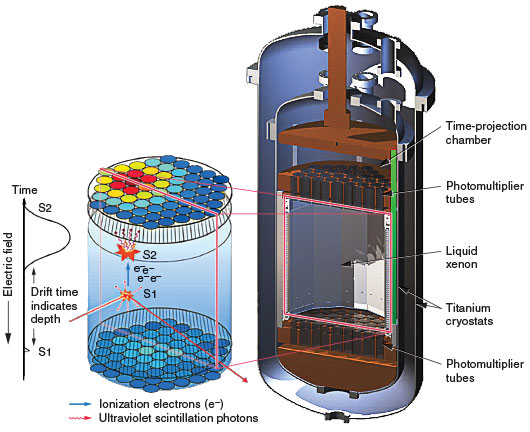
\includegraphics[scale=0.25]{lux.jpg}
\caption{Image depicting the internals of the LUX detector.}
\label{fig:LUX}
\end{figure}

In order to distinguish dark matter signals in the detector from background signals the detector's response to nuclear recoil events and electron recoil events must be well understood. For calibrating electron recoil events it is common to use an external beta emitter such as cesium-137.  However, the xenon in LUX has a strong self-shielding characteristic at UV wavelengths.  While this is convenient for eliminating background radiation, it creates a challenge for calibrating the innermost regions of a detector the size of LUX.

To overcome this problem the LUX collaboration is making use of internal calibration sources.  An ideal internal calibration source would need to be a single beta emitter in the energy range of interest ($ <15 $ keV) which can be dissolved into the liquid xenon in the detector.  Furthermore, the source must be made of a material with low electronegativity so that it will not poison the detector's charge drift length.  Similarly the source cannot attenuate the UV scintillation light produced by events in the detector.  To achieve a reliable calibration in all regions of the detector the source would need to have a long enough life time to diffuse throughout the entire detector (a few hours).  Finally, there must be a method for removing the source once the calibration has finished.  This could simply mean waiting for the source to decay if its half life is short, or actively purifying the source out of the detector if its half life is long \cite{Kastens}.

Tritium meets several of these requirements.  It is a beta emitter with a Q-value of 18 keV that produces a broad spectrum over the entire energy range of interest.  Its 12.3 year half life means that the source will have plenty of time to dissolve uniformly throughout the detector.  However, this long half life is potentially dangerous, since one can not simply wait for it to decay away -- it must be actively removed from the detector when the calibration is completed.  To complicate this matter bare tritium sticks to most surfaces, including materials like teflon, polyethylene, and steel which make up the majority of most xenon detectors.

To make tritium removal more feasible we have made use of tritiated methane (CH$_3$T).  Methane is highly inert due to its fully saturated carbon-hydrogen bonds.  It has a diffusion constant in polyethylene that is 10 times smaller than hydrogen, and it does not capture electrons that will be drifting through the detector.  By replacing one of the hydrogen atoms in a methane molecule with tritium we combine the strength of both of these materials, resulting in the ideal internal calibration source.